\documentclass[10pt,twocolumn,letterpaper]{article}

\usepackage{cvpr}
\usepackage{times}
\usepackage{epsfig}
\usepackage{graphicx}
\usepackage{amsmath}
\usepackage{amssymb}
\usepackage[euler]{textgreek}

% Include other packages here, before hyperref.

% If you comment hyperref and then uncomment it, you should delete
% egpaper.aux before re-running latex.  (Or just hit 'q' on the first latex
% run, let it finish, and you should be clear).
\usepackage[pagebackref=true,breaklinks=true,letterpaper=true,colorlinks,bookmarks=false]{hyperref}

\cvprfinalcopy % *** Uncomment this line for the final submission

\def\cvprPaperID{****} % *** Enter the CVPR Paper ID here
\def\httilde{\mbox{\tt\raisebox{-.5ex}{\symbol{126}}}}

% Pages are numbered in submission mode, and unnumbered in camera-ready
\ifcvprfinal\pagestyle{empty}\fi

\begin{document}

%%%%%%%%% TITLE
\title{Deep Reinforcement Learning for Futures Trading}

\author{Niklas Lifors\\
Georgia Institute of Technology\\
Atlanta, GA\\
{\tt\small nlifors3@gatech.edu}\\
{\tt\small Code Repo: https://github.com/nlifors/DeepTrader}
% For a paper whose authors are all at the same institution,
% omit the following lines up until the closing ``}''.
% Additional authors and addresses can be added with ``\and'',
% just like the second author.
% To save space, use either the email address or home page, not both
% \and
% Second Author\\
% Institution2\\
% First line of institution2 address\\
% {\tt\small secondauthor@i2.org}
}

\maketitle
%\thispagestyle{empty}

%%%%%%%%% ABSTRACT
\begin{abstract}
   In this project, we implement a deep reinforcement learning 
   ("DRL") agent that learns how to enter and exit positions in a variety 
   of futures markets. The deep learning network architecture is varied to
   determine the impact on the agent's performance when using either a 
   linear, fully connected network or an LSTM architecture. In addition,
   the DRL environment and reward function are designed such that the
   agent receives historical information about changes in price and price-
   derived indicators, but using no other human-introduced biases in the
   reward function to fully allow the agent to explore and learn independently.
\end{abstract}

%%%%%%%%% BODY TEXT
\section{Introduction}
The trading of financial instruments for speculation has since the formation of exchanges been approached by individuals and companies attempting to profit from the daily price fluctuations, often with great difficulty due to the near-stochastic movement of prices. Many theories, methodologies and strategies have been applied in an effort to gain an advantage in the markets, and the calculation and study of price-derived indicators, which often synthesize the time-based changes in prices into more understandable trend lines and momentum signals, has been widely popular in recent decades.

Recent advances in applied machine learning to make predictions on large data sets provide another set of tools for making investment decisions. More specifically, deep learning and the use of reinforcement learning to allow an agent to act independently without specific instructions on what to focus on, has the potential to make large improvements in how decisions are made to enter and exit financial instrument holdings. 

In contrast to many other studies on stock market investing which primarily consider long positions only, this study uses futures contracts to also allow the agent to operate on the short side, which is beneficial in non-directional markets such as currencies and cyclical commodities. If this methodology proves successful, it can have significant impacts on how both games and markets that have a large stochastic component are approached.

This project attempts to implement such an agent that can make profitable buy, sell and hold decisions for a representative selection of futures markets. To accomplish this, the agent will need an environment to operate in, including a reward function that will provide enough incentive for the agent to learn to seek profitable positions to enter, avoid large holding losses, and ultimately exit a position at a profit. This study will emphasize and explore the importance of the chosen deep learning architectures, and will make certain initial assumption regarding the Reinforcement Learning algorithm that will be used throughout the experiments.

\subsection{Data}
To train the agent, historical daily price data was used which includes data attributes representing each day's open, close, high and low price for the prior 4 years, dating from 7/10/2017 to 11/23/2020, comprising 1028 rows of data for each financial instrument included in the training. The historical price data sets were obtained from Yahoo Finance, and consisted of price data for the continuous future contracts. The futures contracts included for training were selected as representational examples comprising stock index futures, interest rate futures, commodity futures and currency futures. By including price data from different types of futures markets, we can better test if the agent is able to learn to operate in different environments of price discovery.

During the data pre-processing stage, the price data was augmented with two price-derived indicators: the Moving Average Convergence and Divergence ("MACD") and the Relative Strength Index ("RSI"). The MACD indicator is used as a general trend indicator, which also includes  information about potential inflection points in a trend, and is calculated as the difference of fast and slow-period exponential moving averages \cite{techanalysis}:
\begin{equation}
MACD = EMA_{12 period} - EMA_{26 period}
\end{equation}
The RSI measures the magnitude of recent price changes, which gives an indication of recent momentum in a given direction, and is calculated as \cite{techanalysis}:
\begin{equation}
RSI = 100 * \frac{up_t(n)}{up_t(n) + down_t(n)}
\end{equation}
where up and down are expressed as the average ratio of upward and downward moves, respectively:
\begin{equation}
up_t(n) = \frac{U_t + U_{t-1} + ... U_{t-n+1}}{n}
\end{equation}
\begin{equation}
down_t(n) = \frac{D_t + D_{t-1} + ... D_{t-n+1}}{n}
\end{equation}
These indicators were added to the data set as calculated values for each day of price data. Since the data sets were used to train a Reinforcement Learning agent, there were no explicit categorical or numerical labels associated with each training example.

Each financial instrument's historical price data was split into a training and test set. The agent was trained on data spanning from 7/10/2017 to 6/30/2019, and the testing was performed on price data from 7/1/2019 to 11/20/2020. By testing the agent on a separate data set we can strictly control that there is no ability for the agent to look forward into the testing price data when training. All reward maximization and neural network loss minimization adjustments were made through architecture revisions and hyper-parameter tuning performed on the training data set only.


%-------------------------------------------------------------------------
%------------------------------------------------------------------------
\section{Approach}

To train and evaluate the agent's ability to learn to trade in the chosen markets, the agent was trained on an evolving architecture, to determine what impact the choice of deep learning architecture, loss function and state complexity had on the results in the performance. For the DRL problem, two main components make up the majority of the characteristics of the solution. First, the reinforcement learning environment defines the state variable and reward function passed back to the agent as it takes actions through each time step in a training episode. The state determines what the agent observers in each time step it interacts with its environment, and needs to encompass all information we wish the agent to consider when making decisions. For this problem, the state is a (1 x 271) tensor, comprising a 90-day look-back period of price changes between time t and t-1, in addition to 90-day histories of the MACD and RSI indicators. The 90-day window provides the agent with a sense of time, such that it can learn to detect important trends in prices and indicator values. Finally, the current position value is added to the state to inform the agent of how well it is doing with respect to its current open position.

\subsection{Reinforcement Learning Algorithm}
The reinforcement learning algorithm used for this study is based on the Q-learning algorithm, which was successfully used to train agents to play various Atari games \cite{playingatari}. Q-learning is concerned with finding the optimal Q-function value, Q*, for any given state and action pair, such that the agent can choose the action that optimizes the sum of future rewards. The Bellman equation for the action-value function, Q, is:
\begin{equation}
Q^*(s,a) = \sum_{s'}Prob(s'|sa) ( Reward^{s'}_{sa} + \gamma  \underset{a}max  Q*(s',a))
\end{equation}
With simple enough state variables over time, an in-memory lookup table can be used for storing the optimal Q-function values derived during training, but for any sufficiently complex state, using a deep neural network to approximate the Q* function has shown great results \cite{playingatari}. For purposes of this study, the Q-learning methodology was used as it has shown to be successful in similar studies for training agents in the financial markets\cite{deep}, and allows us to fix the algorithm type while focusing on studying the impact the choice of the deep neural network architecture has on the agent's performance.

\subsection{DQN Neural Network ("Q-Network")}
The deep neural network was implemented with PyTorch, using the library's \emph{torch.nn} layers and loss functions. The Adam optimizer was used for all experiments, due to its generally good performance with multi-layer networks trained on large data sets \cite{adam}.
The learning rate was also fixed across experiments, set to a sufficiently course value of 0.001 to force a quicker convergence given the limited number of training episodes included for comparative purposes to manage the overall training time for each experiment. Based on trial runs using longer episode lengths in the 500-1000 range, most training efforts resulted in a degradation in performance past approximately 200 episodes.

For the Q-network update iteration, we get the network's estimated Q value and compare it to the optimal Q value based on equation 5 above. The estimated and calculated Q-values are fed into the loss function, which is then back-propagated through the network layers to update the learned weights for all linear, non-linear activations and LSTM layers. Since we are comparing actual Q-values, and not probability distributions over categories, the Mean Squared Error loss function is appropriate, and will be used throughout the experiments. However, in early episodes when the estimated and calculated Q-values show larger differences, such as when the reward function can vary widely, there is potential for noisy error calculations and resulting gradients. To alleviate this, we will perform a test comparison using using the Huber loss function, which switches to a Mean Absolute Error for large errors, but uses the MSE for smaller error \cite{huberloss}.

For the network architecture, two types of networks will be compared. First, a network with fully connected linear layers and activation functions will be used as a baseline, to establish the feasibility of training the agent to achieve acceptable results (Figure 1). 

\begin{figure}[hbt!]
    \begin{center}
    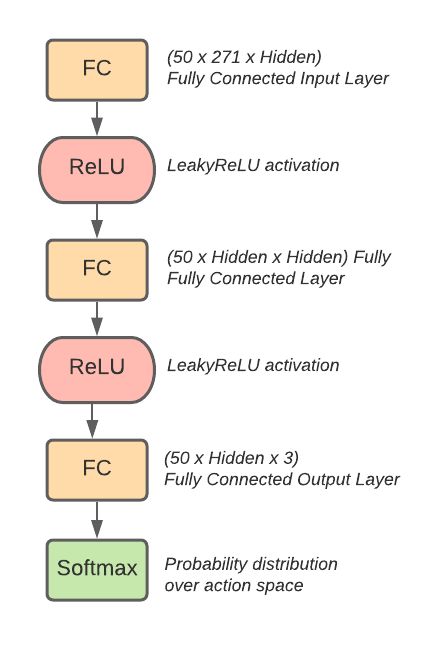
\includegraphics[scale=0.7]{linear.png}
    \caption{Linear neural network architecture.}
    \end{center}
\end{figure}

Since financial price data evolves in a time-series, where each successive price at time t evolves, with a stochastic element, from the prior price at time t-1, the LSTM architecture appears to be a suitable model, based on its use of a memory cell to retain information from one training epoch to the next. To see if an LSTM model improves on the agent's ability to detect price discovery patters over time, an LSTM layer was introduced to the architecture (Figure 2). Finally, the Softmax function gives us a probability distribution over the allowed action space (3 actions).

\begin{figure}[hbt!]
\begin{center}
     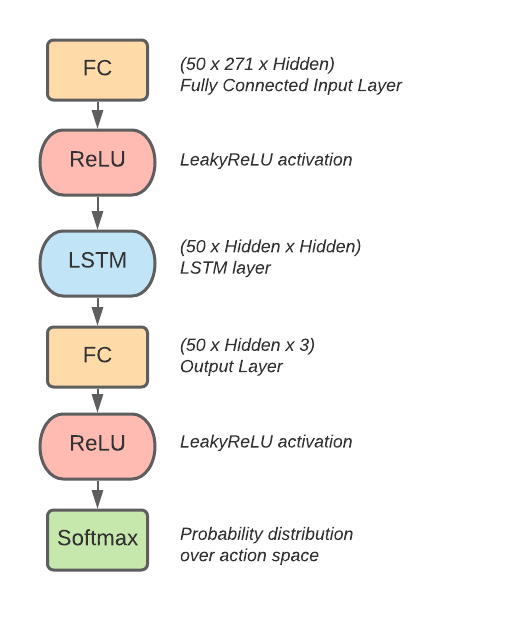
\includegraphics[scale=0.7]{lstm.png}
     \caption{LSTM neural network architecture.}
\end{center}
\end{figure}

When representing the state variable used as the input, X, to the model, the initial approach was to use the current episode's price at time t only, without consideration for prior prices or indicator values. Using this state in early training runs, the agent's reward over time did not improve, nor did the loss reduce of training episodes. To improve on the state representation, an existing environment implementation code base was used as a reference\cite{valuebased} which used a 90-day look-back period of changes in price from t-1 to t. In addition to this baseline state, the indicator values from Equation 1 and 2 were added with the same 90-day look-back period. With these changes to the state, the agent was able to learn over time, and show a continuous improvement in the accumulated reward.

The network depths were kept relatively shallow, since more layers tend to over-fit, given the additional representational power provided by the additional layers to fit the function. Given that financial time-series data with a stochastic element is very sensitive to over-fitting when approximated by any type of predictive models, the smaller network sizes were used as a precaution. The main Q-network was updated from a running memory of past observations, where the training batch was sampled randomly from memory. This is a common technique \cite{playingatari}, called memory replay, that mitigates training the network on sequential, and highly dependent, state input data. Based on the results, significant over-fitting did not prove to be a problem, and the model was able to generalize well into the unseen testing data set.

In addition to the main Q-network used for training, a secondary copy of the Q-network, often referred to as the target network, was used\cite{theoreticaldqn}. The target network is used for generating the Q-value estimate, and is kept separate from the training network to so as not to train the network using values derived from it in the current iteration. The target network is copied from the training network after \texttau\ number of training iteration, inheriting the exact architecture and weights at point of freezing using a deep copy of the source network.

\section{Experiments and Results}

\begin{table*}
\begin{center}
\begin{tabular}{|l|c|c|c|c|c|c|c|}
\hline
Experiment Name & Reward Function & Network & Loss Function & Hidden Size & Batch Size & LR & \texttau\\
\hline\hline
Baseline Long Only & Binary: +1/-1 & Fully Connected & MSE & 100 & 50 & 0.001 & 100 \\
Baseline Long Short & Binary: +1/-1 & Fully Connected & MSE & 100 & 50 & 0.001 & 100 \\
LSTM & Binary: +1/-1 & LSTM & MSE & 100 & 50 & 0.001 & 100 \\
LSTM Stop Loss & Trade P\&L & LSTM & Huber & 100 & 50 & 0.001 & 100 \\
\hline
\end{tabular}
\end{center}
\caption{Experiment Hyper-Parameters.}
\label{tab:contributions}
\end{table*}

To test the performance of the agent over different network architectures, four experiments were conducted with varying models and environments. Each experiment was trained over 100 episodes of training, with each episode walking through the full historical training data from start to end. Within each episode, the Q-network was trained in incremental batches of 50 random samples once the observation memory had been filled (200 state observation capacity). The training log provided each episodes average rolling reward and loss along with the GPU-enabled training time. Once trained, the model's parameters were saved, and the test run was performed on the out-of-sample test periods. The test run provided the final trades taken, their net P\&L, and the daily valuation of realized and unrealized gains and losses.

\begin{figure}[hbt!]
\begin{center}
     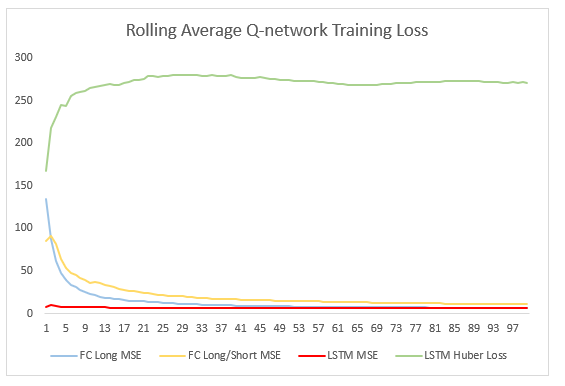
\includegraphics[scale=0.54]{average_loss.PNG}
     \caption{Rolling Average Q-Network Training Loss for RTY Contract.}
\end{center}
\end{figure}
\begin{figure}[hbt!]
\begin{center}
     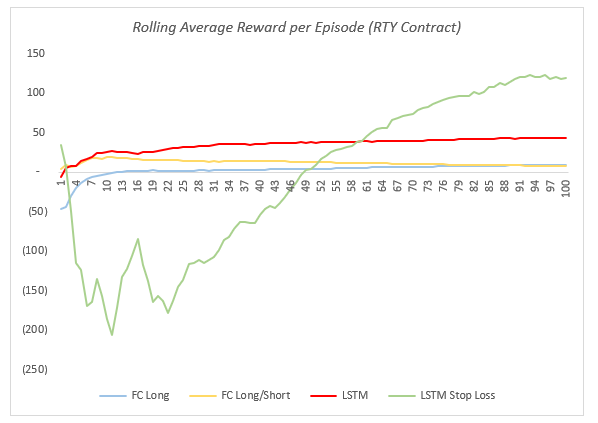
\includegraphics[scale=0.52]{average_reward.PNG}
     \caption{Rolling Average Reward per Episode for RTY Contract.}
\end{center}
\end{figure}

The first baseline experiment was conducted to establish the general feasibility of training an agent to trade the chosen markets. The baseline included fully connected layers with ReLU activations (Figure 1), and the agent was allowed to only take long positions, similar to other studies performed for stock market trading simulations \cite{ensemble}. The training results for the chosen network and input values show a smooth decreasing and converging loss curve, in addition to an increasing average episodic reward to just over the positive x-axis. The profitability curve for closed trades (Figure 3) show promising regions of increasing profits, but the agent experiences a large draw-down around April 2020 due to the large crash in oil prices at that time. Overall, the agent was not able to recover to a net positive portfolio balance at the end of the testing period.

The next experiment maintained the same Q-network architecture, but now allowed the agent to both enter long and short positions. The shape of the reward, loss and profitability curves are similar to the long-only agent, but the ability to take short positions increased the episodic training reward, which also translated to an upward shift in the realized gain and portfolio balance curve. Again, the crude oil market proved problematic, as the agent held a long position during the April market crash that saw prices going into negative values.

\begin{table*}
\begin{center}
\begin{tabular}{|l|c|c|c|c|c|c|c|}
\hline
Ticker & Contract Name & Point Value (\$) & FC Long Only & FC Long Short & LSTM & LSTM Stop Loss \\
\hline\hline
6E & Euro FX & 125,000 & 456 & 1,043 & \textbf{5,137} & 0* \\
CL & Crude Oil & 1,000 & (66,290) & (30,890) & 6,860 & \textbf{88,110} \\ 
GC & Gold & 100 & 35,670 & \textbf{65,320} & 44,710 & 29,690 \\
LE & Live Cattle & 400 & 6,620 & \textbf{11,050}& 5,960 & (3,330) \\
RTY & Russell 2000 & 50 & (12,186) & (4,775) & 8,040 & \textbf{20,405} \\
ZN & 10-Year Note & 1,000 & \textbf{14,469} & (550) & (798) & 7,453 \\

% Team Member 1 & Data Creation and Implementation & Scraped the dataset for this project and trained the CNN of the encoder. \\
% Team Member 2 & Implementation and Analysis & Trained the LSTM of the encoder and analyzed the results. \\
\hline
\end{tabular}
\end{center}
\caption{Experiment Results: Testing Period Closed Trade P\&L (in US\$) Per Contract. *The agent did not generate any trades for the Euro FX contract under the LSTM Stop Loss environment. }
\label{tab:contributions}
\end{table*}

To test the hypothesis that the LSTM architecture with its hidden cell state can hold a belief about changes in historical price states, the next experiment swapped out the architecture only (Figure 2), while retaining the exact same environment and reward function. Without any other changes, the agent was now able to use the provided 90-day price and indicator value histories to better effect, as is shown by the very smoothly upward trending closed trade curve. However, due to the reward function, which rewards the agent for profitable closed trades, but doesn't punish for large unrealized losses, the agent experienced a large draw-down period during the crude oil volatility, which impacted only the open trade balance but left the closed trade curve untouched.

To remedy the problem of large open trade unrealized losses, the final experiment included an additional environment constraint to automatically close any open trades exceeding an unrealized loss of 5\% of the market value. To prompt the agent to work around this constraint, the reward function was modified to forgo the binary reward and instead set the reward equal to the closed trade P\&L, in addition to including the total portfolio's balance (realized and unrealized) as a state variable. Perhaps due to the wide range of rewards returned, which adds instability to the calculated q-values for each state, the MSE loss function returned large and diverging loss numbers. However, when switching to the Huber loss function, the loss range now stabilized throughout the training episodes to a more normal range not far from those seen for the prior experiments. This shows that the Huber loss function can help dampen the impact of training the network using largely fluctuating state tensors and resulting target Q-values.

Using this environment configuration coupled with the LSTM architecture and Huber loss function, the agent shows its most profitable behavior, and is even able to position itself on the right side (short position) of the large down move in the crude oil market. Even without this outlier trade, both the closed trade realized and portfolio balance curves show strong upward trends throughout the testing period. Also possibly due to the forced stop loss condition, the agent has far more executed trades during the testing period than any of the other experiments (Figure 3).

\begin{figure}[hbt!]
\begin{center}
     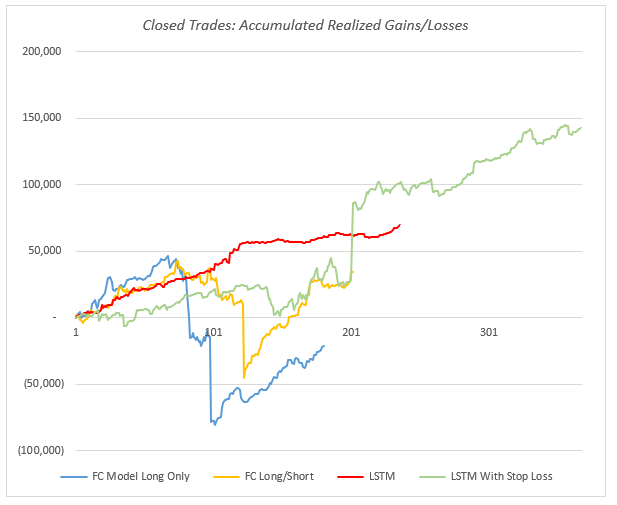
\includegraphics[scale=0.52]{closed_trades.PNG}
     \caption{Closed Trades: Accumulated Realized Gains. Difference in curve lengths due to actual number of trades taken.}
\end{center}
\end{figure}

\begin{figure}[hbt!]
\begin{center}
     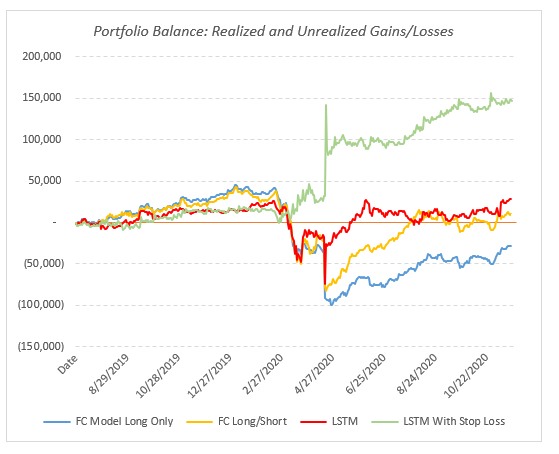
\includegraphics[scale=0.57]{portfolio_balance.PNG}
     \caption{Portfolio Balance by Date: Combined Realized and Unrealized.}
\end{center}
\end{figure}

\begin{table*}
\begin{center}
\begin{tabular}{|l|l|}
\hline
Student Name & Contributed Aspects and Details\\
\hline\hline
Niklas Lifors & Data sourcing and pre-processing logic.\\
& Customization and extension to reinforcement learning library.\\
& Design and implementation of deep neural networks for Q-function approximation.\\
& Conducting of experiments, compiling results and report writing.\\
\hline
\end{tabular}
\end{center}
\caption{Contributions of team members.}
\label{tab:contributions}
\end{table*}

\section{Future Improvements}

A number of additional improvements can be made to enhance the performance of an auto-trading deep reinforcement learning agent. First, the training environment can be improved in a number of ways. Primarily, the agent needs to be able to consider the open unrealized gains or losses when evaluating the actions to take. This can be accomplished by shaping the reward in such a way that a large unrealized loss incurs a penalty, which would drive the agent to avoid those state conditions. Another solution is to expand the action space with additional opportunities for the agent to mitigate an unrealized loss possibly using options on the underlying futures contract. Opening up the option space would massively increase the state and action space, however, due to the number of potential option positions that can be entered into, when options spreads are included.

To improve the agent's learning capacity, an exploration can be made in increasing the layers of the network. For LSTM architectures, multiple LSTM layers can be added, or stacked, to increase the representational power of the network to learn the additional complexity of the environment's state. There has been some success using stacked auto-encoders prior to the LSTM layer in improving the t+1 price forecasting \cite{stackedlstm}. An interesting opportunity exists to include a separate LSTM model with such a stacked architecture to predict the next day's price as an additional component of the state variable. 

A third improvement includes experimenting with other architectures, such as the transformer model, that has shown great success in replacing RNN and LSTM architectures for text processing. Some early attempts to use transformers for the reinforcement learning deep neural network have yielded limited success, due to the transformer model being too unstable to properly learn, but architecture modifications, such as the reordering of normalization layers, have shown better results.\cite{transformers}. Given the remarkable performance on other sequential and time-based data sets, transformer architectures such as GPT-3 could be strong candidates for applying to price prediction and time-series dependent state representations used for the reinforcement learning networks.

\section{Conclusion}
In this project, we attempted to train a deep reinforcement learning agent to profitable decide when and how to enter a position in a handful of representative futures markets. Using a DQN RL architecture coupled with an LSTM deep neural network model, the results show that an agent can be trained to profitably trade certain instruments. Even without generalizing across markets, there is an opportunity to apply models specifically trained for certain markets to exploit the price movement characteristics of individual markets. By using an LSTM model that incorporates a memory cell, the agent has show to be better equipped to learn an environment state that is time-based.

{\small
\bibliographystyle{ieee_fullname}
\bibliography{egbib}
}

\begin{thebibliography}{9}

\bibitem{techanalysis} 
Ko Chiu Yu
\textit{Technical Analysis with R (Second Edition)}. 
https://bookdown.org/kochiuyu/technical-analysis-with-r-second-edition/

\bibitem{playingatari} 
Volodymyr Mnih and Koray Kavukcuoglu and David Silver et al.
\textit{Playing Atari with Deep Reinforcement Learning}. 
DeepMind Technologies

\bibitem{deep} 
Zihao Zhang, Stefan Zohren, and Stephen Roberts
\textit{Deep Reinforcement for Trading}. 
University of Oxford

\bibitem{adam} 
Diederik P. Kingma and Jimmy Lei Ba
\textit{Adam: A Method For Stochastic Optimization}. 
OpenAI, University of Toronto

\bibitem{huberloss} 
Scott Fujimoto, David Meger, Doina Precup
\textit{An Equivalence between Loss Functions and Non-Uniform Sampling in Experience Replay}. 
Mila, McGill University

\bibitem{valuebased} 
Jay Chan Hoi
\textit{Value Based Deep Reinforcement Learning Trading Model in Pytorch}. 
https://github.com/JayChanHoi/value-based-deep-reinforcement-learning-trading-model-in-pytorch

\bibitem{theoreticaldqn} 
Jianqing Fan and Zhaoran Wang and Yuchen Xie and Zhuoran Yang∗
\textit{A Theoretical Analysis of Deep Q-Learning}. 
Princeton University, NJ

\bibitem{stackedlstm} 
Wei Bao and Jun Yue and Yulei Rao
\textit{A deep learning framework for financial time series using stacked autoencoders and longshort term memory}.
Princeton University, NJ

\bibitem{transformers} 
Emilio Parisotto and H. Francis Song and Jack W. Rae et al.
\textit{Stabilizing Transformers for Reinforcement Learning}.
DeepMind, London, UK

\bibitem{ensemble} 
Hongyang Yang and Xiao-Yang Liu and Shan Zhong and Anwar Walid
\textit{Deep Reinforcement Learning for Automated Stock Trading: An Ensemble Strategy}.
Columbia Univerisy, NY.

\end{thebibliography}

\end{document}